\documentclass[border=2pt]{standalone}
\usepackage{pgfplots}\pgfplotsset{compat=1.18}\usepackage{amsmath}
\begin{document}
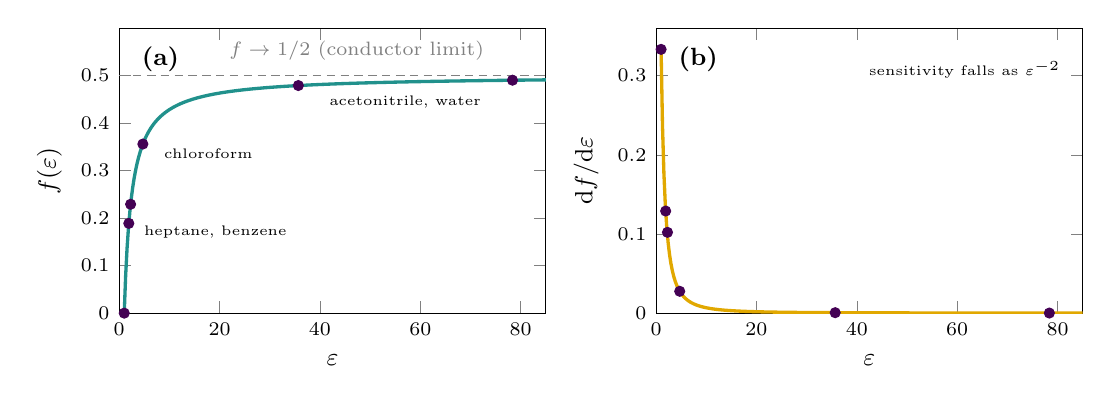
\begin{tikzpicture}
  \definecolor{c1}{HTML}{440154}\definecolor{c2}{HTML}{21918C}\definecolor{c3}{HTML}{E1A800}
  \pgfplotsset{every axis/.append style={width=7cm,height=5.2cm,
    tick label style={font=\scriptsize},label style={font=\small},
    tick align=inside,mark size=1.8pt}}

  \begin{axis}[name=a, xlabel={$\varepsilon$}, ylabel={$f(\varepsilon)$},
      xmin=0, xmax=85, ymin=0, ymax=0.60, ytick={0,0.1,0.2,0.3,0.4,0.5}]
    \addplot[gray, densely dashed, domain=0:85, forget plot] {0.5};
    \node[font=\scriptsize, color=gray, anchor=south west] at (axis cs:20,0.512) {$f \to 1/2$ (conductor limit)};
    \addplot[c2, very thick, domain=1:85, samples=300, forget plot] {(x-1)/(2*x+1)};
    \addplot[only marks, mark=*, c1] coordinates {
      (1,0) (1.9113,0.1890) (2.2706,0.2293) (4.7113,0.3561)
      (35.688,0.4793) (78.3553,0.4905)};
    \node[font=\tiny, anchor=west] at (axis cs:3,0.17) {heptane, benzene};
    \node[font=\tiny, anchor=west] at (axis cs:7,0.335) {chloroform};
    \node[font=\tiny, anchor=east] at (axis cs:74,0.445) {acetonitrile, water};
    \node[font=\small\bfseries, anchor=north west] at (rel axis cs:0.03,0.97) {(a)};
  \end{axis}

  \begin{axis}[at={(a.east)}, anchor=west, xshift=1.4cm,
      xlabel={$\varepsilon$}, ylabel={$\mathrm{d}f/\mathrm{d}\varepsilon$},
      xmin=0, xmax=85, ymin=0, ymax=0.36, ymode=normal]
    \addplot[c3, very thick, domain=1:85, samples=300, forget plot] {3/(2*x+1)^2};
    \addplot[only marks, mark=*, c1] coordinates {
      (1,0.3333) (1.9113,0.1290) (2.2706,0.1021) (4.7113,0.0276)
      (35.688,0.00057) (78.3553,0.00012)};
    \node[font=\tiny, anchor=north east, align=right] at (rel axis cs:0.97,0.92)
      {sensitivity falls as $\varepsilon^{-2}$};
    \node[font=\small\bfseries, anchor=north west] at (rel axis cs:0.03,0.97) {(b)};
  \end{axis}
\end{tikzpicture}
\end{document}
